\documentclass[../main.tex]{subfiles}

\begin{document}
In the algorithm's assessment, three carefully chosen \gls{cryoem} datasets have been used. The datasets reflect various conditions that can be found in reality, so that the comparisons shown here are transcendental. One the datasets exhibits compositional heterogeneity, while the other two are highly flexible. In such a way, we intend to assess the performance in both heterogeneity scenarios.

We have preferred to use publicly available datasets from \gls{empiar}, so that the results detailed here can be replicated. Nevertheless we have also used a in-house acquisition that is not public yet (although it is expected to become public soon).

\subsection{TRPV-5}
The Transient Receptor Potential Vanilloid 5 (TRPV-5) protein is a ion channel, which plays a crucial role in the regulation of calcium homeostasis within various tissues and cells. This sort of channels are widely distributed in mammalian organisms and are involved in sensory perception, cell signaling, and the maintenance of cellular ionic balance. TRPV-5 is primarily expressed in the renal tubules, where it participates in the reabsorption of calcium ions. The protein's significance in renal physiology underscores its role in maintaining systemic calcium levels, ultimately impacting bone health, neuromuscular function, and overall mineral homeostasis.

Research on TRPV-5 has gained significance in recent years, focusing on its structural features, functional properties, and the signaling pathways it engages in. Understanding the molecular behaviour of TRPV-5 provides a basis for developing targeted therapies for disorders related to calcium deregulation.

We have decided to mix two \gls{empiar} entries where one of them comes from an experiment where calmodulin was added in-vitro (EMPIAR-10253) and potentially binds to two N and C lobes. The other experiment comes from a mutant in a clean buffer, although it had potential to bind endogenous calmodulin (EMPIAR-10256). Unlike the first experiment, the mutation on the TRPV-5 from the second experiment disables the calmodulin binding in the C lobe. Therefore, the difference between the two datasets lies around the binding site in the C lobe\cite{zhou2022}\cite{dang2019}. These lobes are highlighted in Figure \ref{fig:5.1:trpv5}.

\begin{figure}[htbp]
    \centering
    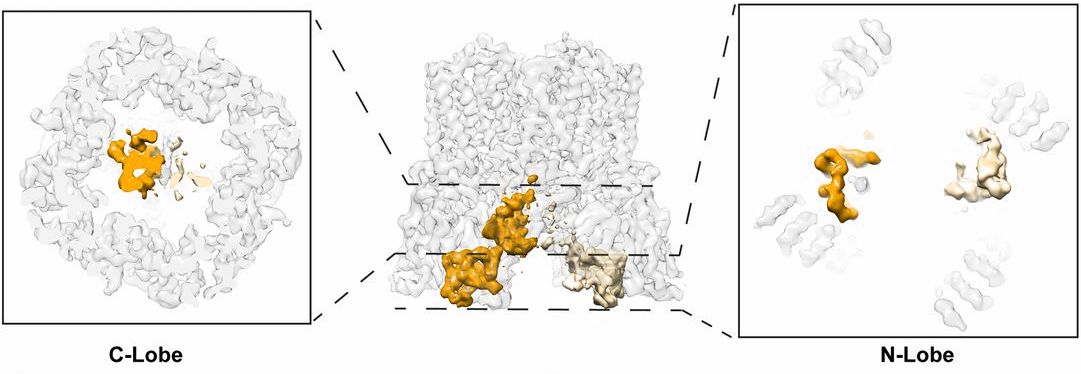
\includegraphics[width=\textwidth]{results/datasets/trpv5}\\
    Image obtained from: \cite{dang2019}
    \caption{TRPV-5 reconstruction}
    \label{fig:5.1:trpv5}
\end{figure}

A similar classification experiment was proposed in the ``Data-driven determination of number of discrete conformations in single-particle cryo-EM'' paper. As stated by its authors, ``These datasets are challenging because the extra density corresponding to calmodulin is very small and breaks the symmetry of the complex making accurate particle alignments critical to achieve a successful separation''\cite{zhou2022}.

The two datasets used in these tests are the EMPIAR-10253\cite{empiar10253} and the EMPIAR-10256\cite{empiar10256}\cite{dang2019}. In conjunction, they sum $166611$ particles, from which $60 \si{\percent}$ originate from the mutant experiment, and the other $40 \si{\percent}$ originate from the in-vitro experiment. These particles have a size of $256 \times 256 \si{px^2}$ and they were acquired with a sampling rate of $1.06 \si{\angstrom/px}$. As two datasets were mixed, it is not fair to consider their alignments, as these were estimated in isolation. Thus, all the particles were re-refined to re-estimate the alignment parameters in heterogenous conditions using Cryosparc's non-uniform refinement\cite{cryosparc}. A sample of the particles of these datasets is showcased in Figure \ref{fig:5.1:trpv5_particles}.
 
\begin{figure}[htbp]
    \centering
    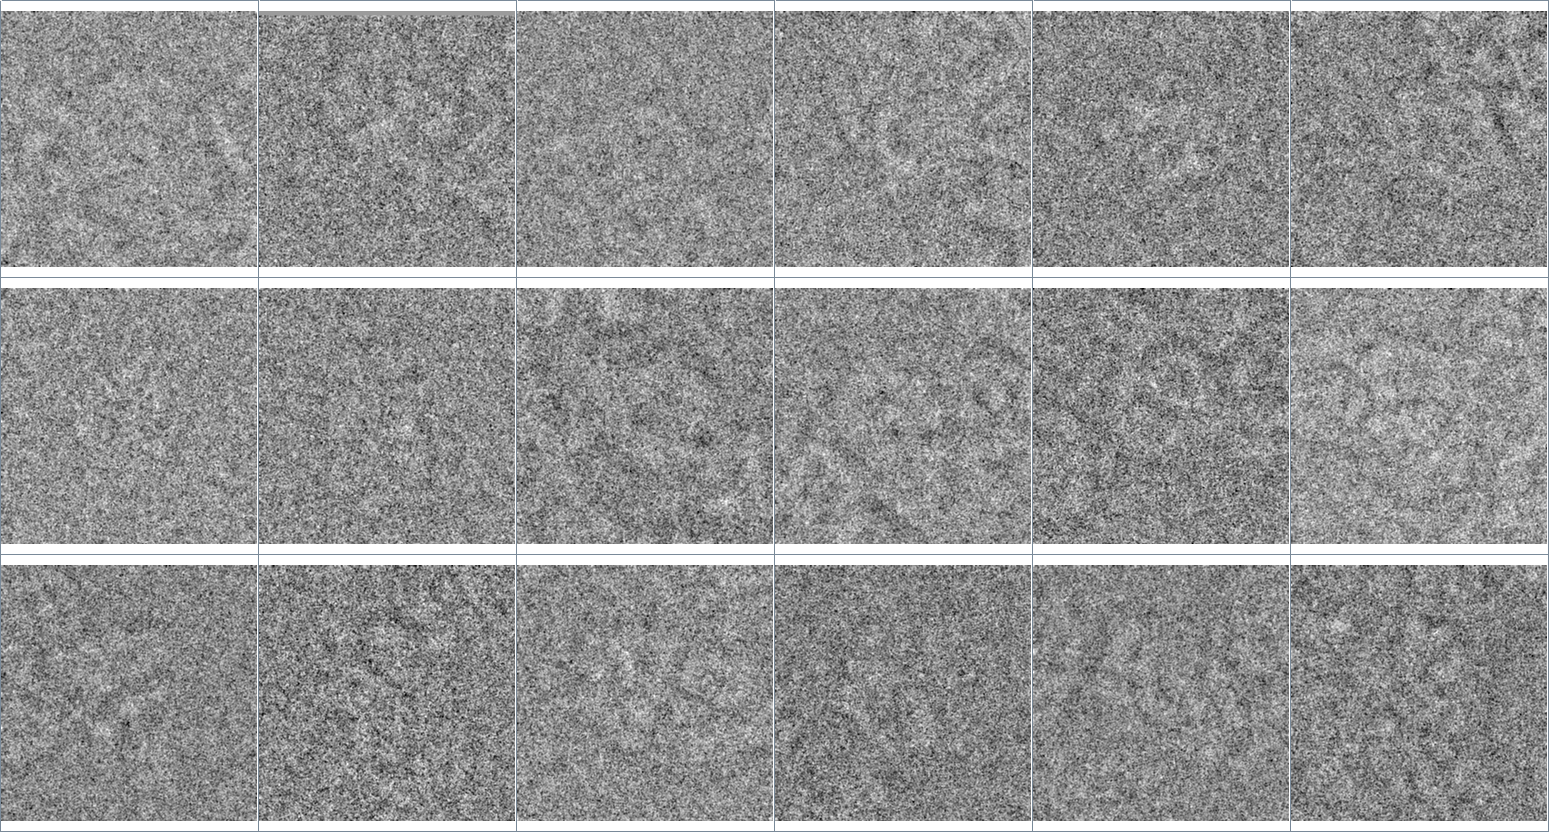
\includegraphics[width=\textwidth]{results/datasets/trpv5 particles}
    \caption{Sample of the TRPV-5 particles}
    \label{fig:5.1:trpv5_particles}
\end{figure}

\subsection{Pre-cathalytic spliceosome}
The pre-cathalytic spliceosome is a critical component in the process of RNA splicing. RNA splicing is a fundamental cellular mechanism that involves the removal of introns (non-coding regions) from precursor messenger RNA (pre-mRNA) and the joining of exons (coding regions) to generate mature mRNA. The spliceosome is a large and dynamic molecular machine responsible for orchestrating this process.

Understanding the functions of the pre-catalytic spliceosome is crucial for unraveling the molecular mechanisms that govern RNA splicing, which plays an important role in gene expression and cellular function. Researchers investigate these processes to gain insights into various genetic and cellular disorders, as abnormalities in splicing can lead to diseases.

This molecular machine is highly flexible, meaning that it exhibits continuous heterogeneity. Indeed, it contains two independent regions with flexibility, which will be analyzed separately. In these analysis we aim to observe multiple stable states on those regions. In particular, we will focus our analysis on the SF3b and helicase regions detailed in Figure \ref{fig:5.1:spliceosome}, which are the most flexible ones. 

\begin{figure}[htbp]
    \centering
    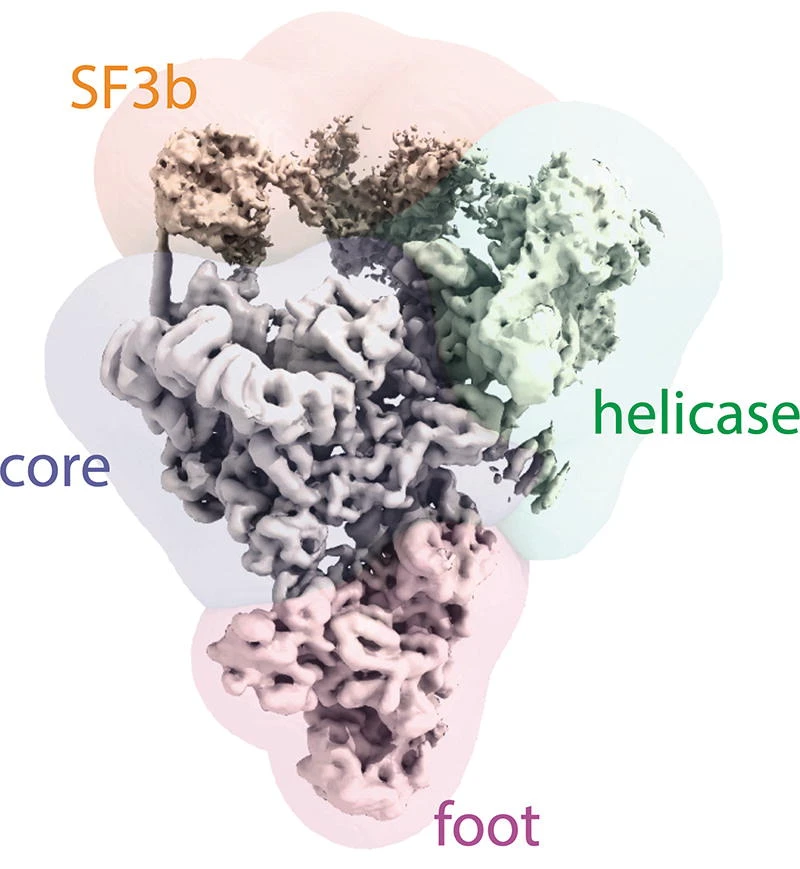
\includegraphics[width=.5\textwidth]{results/datasets/spliceosome}\\
    Image obtained from: \cite{nakane2021}
    \caption{Pre-cathalytic spliceosome reconstruction}
    \label{fig:5.1:spliceosome}
\end{figure}

We have conducted our tests on this macro-molecule using the publicly available a public dataset from the \gls{empiar} repository, precisely the EMPIAR-10180\cite{empiar10180} dataset. This dataset is commonly used as a baseline to assess and evaluate flexibility analysis algorithms\cite{herreros2021}\cite{nakane2021}\cite{herreros2023}. Due to this continuous heterogeneity, the our aim is to observe the most common states. The EMPIAR-10180 dataset is provided as a set of $327490$ aligned particles of size $320 \times 320 \si{px^2}$ at a sampling rate of $1.699 \si{\angstrom}$. Additionally, the authors of the dataset also provide masks enclosing the \glspl{roi} of each of the flexible regions. A sample of the particles of this dataset is displayed in Figure \ref{fig:5.1:spliceosome_particles}.

\begin{figure}[htbp]
    \centering
    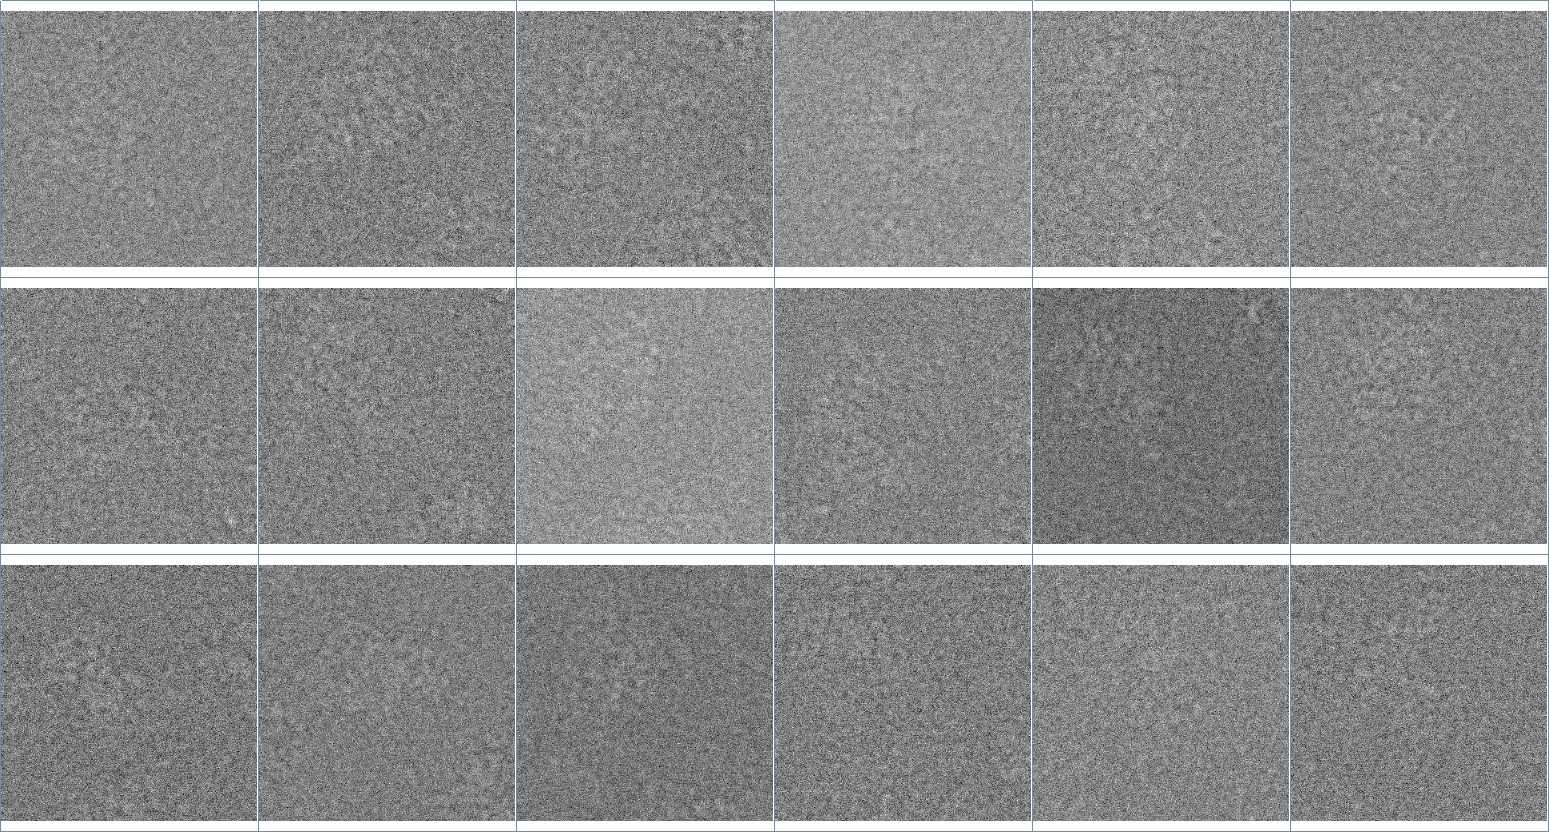
\includegraphics[width=\textwidth]{results/datasets/spliceosome particles}
    \caption{Sample of the spliceosome particles}
    \label{fig:5.1:spliceosome_particles}
\end{figure}

\subsection{HER-2}
The HER-2 protein, also known as human epidermal growth factor receptor 2, is a crucial molecule in the context of cell growth, division, and differentiation. HER-2 is particularly remarkable for its involvement in cancer biology, as its overexpression or amplification has been identified in a variety of malignancies, most notably breast cancer. When HER-2 is overexpressed, it can lead to uncontrolled cell proliferation, increased survival, and enhanced invasive properties, contributing to the aggressive nature of certain cancer types.

\begin{figure}[htbp]
    \centering
    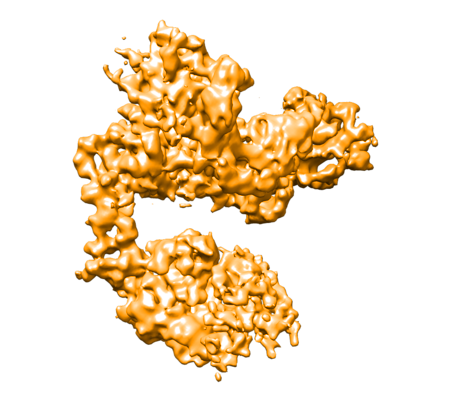
\includegraphics[width=.5\textwidth]{results/datasets/her2}
    \caption{HER-2 reconstruction}
    \label{fig:5.1:her2}
\end{figure}

In the results detailed on this chapter, we have experimented with a in-house dataset which was previously processed by Dr. Marcos Gragera Cabezudo. This dataset is comprised of $352500$ aligned particles of size $200 \times 200 \si{px^2}$ acquired with a sampling rate of $1.3 \si{\angstrom/px}$. A sample of these particles is shown in Figure \ref{fig:5.1:her2_particles}. Similarly to the pre-cathalytic spliceosome, HER-2 also exhibits flexibility. In particular, it is comprised of two sub-units that are flexibly connected. Thus, by performing a 3D classification on it, we aim to observe multiple states.

\begin{figure}[htbp]
    \centering
    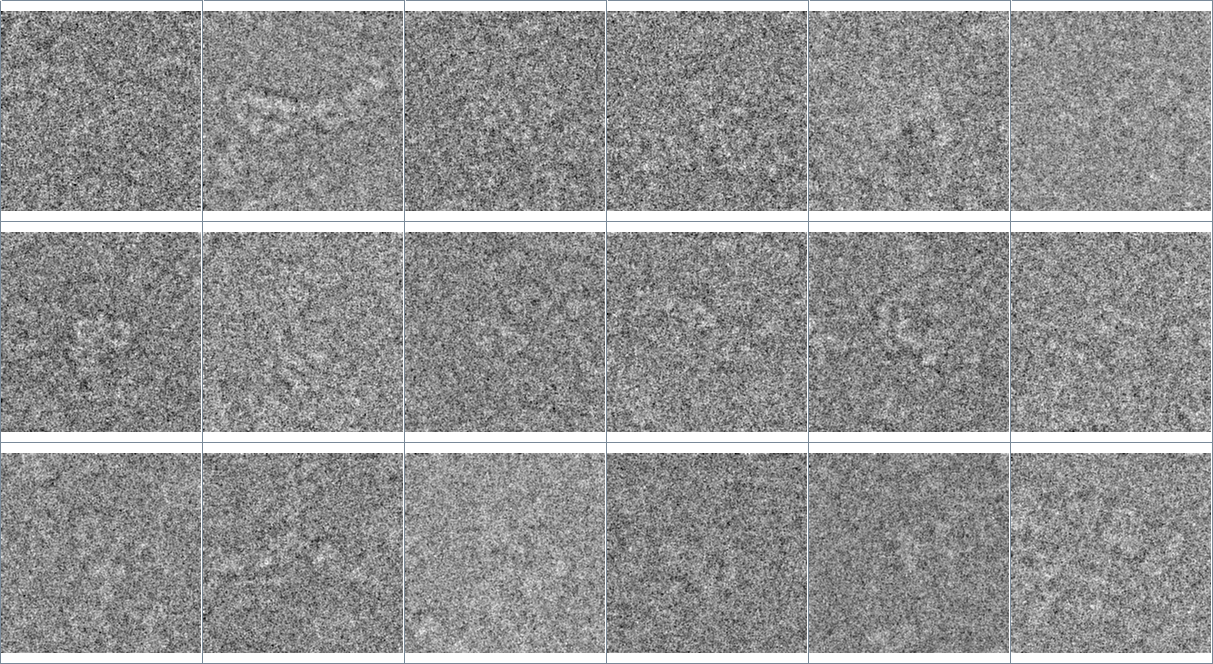
\includegraphics[width=\textwidth]{results/datasets/her2 particles}
    \caption{Sample of the HER-2 particles}
    \label{fig:5.1:her2_particles}
\end{figure}

\end{document}
